\documentclass[11pt]{article}
\usepackage{graphicx}  % this is the up-to-date package for all figures
\usepackage{float}	% allows use of 'H' command
\usepackage{hyperref}	% needed to add hyperlinks
\hypersetup{
  colorlinks=true,
  linkcolor=blue,
  filecolor=magenta,
  urlcolor=cyan,
}

% these are some custom control of the page size and margins
% \topmargin= 0.2in  % these 1st two may be needed for some computers
%\textheight=8.75in
\textwidth=6.5in
\oddsidemargin=0cm
\evensidemargin=0cm

% this is where the actual document itself (rather than control statements) begins:

\begin{document}

\pagestyle{myheadings}


\title{Projectile Motion:\\
No-Dong Missile}


\author{Corey Mutnik \\
{\it Computational Physics 305, University of Hawaii at Manoa} }


\date{April 7, 2015}

\maketitle   




\abstract{
Missiles launch from a surface using a propellent to accelerate.  The duration of 
time during which a propellent is ignited, a burn time, determines the distance any such missile 
is able to travel.  A single stage missile has one burn time.  By accurately modeling the burn time the 
motion of such a rocket can be determined.
}

\section{Introduction}
From Newton's Second Law we know that the net force on an object is the rate of change of its 
momentum with respect to time.  After little manipulation we can rewrite this force law to 
determine a characteristic equation for acceleration.  Once this is done we are able to use 
computational methods, such as Runge-Kutta, to achieve numerical approximations that model system 
solutions.  
\begin{equation}
\label{acceleration}
\frac{d\vec{v}}{dt} ~=~ \frac{1}{m(t)}
                            \left [ \vec{F}_g(\vec{r}(t)) + 
                            \vec{F}_b(\vec{v}(t)) + 
                            \vec{F}_p(m(t)) \right ]
\end{equation}
where m(t) is the time dependent mass, $\vec F_{g}$ is the force due to gravity, $\vec F_{d}$ is 
the force due to drag, and $\vec F_{p}$ is the force given to the rocket as a result of its 
thrust.  The forces summed here are dependent on $\vec{r}(t)$, $\vec{v}(t)$, and m(t).  Here $\vec{r}(t)$ 
is the 3-vector pertaining to the projectiles position, relative to the center of the Earth.  The objects 
velocity is denoted by $\vec{v}(t)$.

\begin{center}
$\vec{F}(\vec{r}) ~=~ -\frac{GMm}{\left |
                    \vec{r}\right|^3} ~ \vec{r}$
\end{center}
where G is the gravitational constant, M is the mass of the Earth, and m is the mass of the modeled 
projectile.
\begin{center}
 $\vec{F}_b ~=~ -b\left
                            |\vec{v}_{app}\right | \vec{v}_{app}$
\end{center}
where $\vec{v}_{app}$ is the apparent velocity of the rocket.  It takes into account the velocity due to 
the rockets motion as well as any needed modification imposed by the wind.  
Here b is Bernoulli's coefficient:
\begin{equation}
\label{dragconst}
 b = C_d A \rho / 2
\end{equation}
where $C_{d}$ is the drag coefficient, A is the cross sectional area, and the air density $\rho$ is 
dependent on the magnitude of the radius vector (as measured from the center of the Earth).



In modeling the 
motion of a rocket it is not sufficient to use mass, one must use time dependent mass.  As a rocket 
burns fuel its mass decreases.  It is evident that once fuel is burned it no longer contributes to the 
mass in need of propulsion; any subsquent burning will be inherently more efficient.  In order to properly 
model such behavior it is necessary to use a function for the mass of a missile rather than a constant 
value.  The mass decreases in a linear fashion:
\begin{center}
 $m(t) ~=~ m_0 - m_{fuel} \frac{t-t_0}{t_b}, ~
                        t<t_b$
\end{center}
\begin{center}
 $m(t) ~=~ m_0 - m_{fuel}, ~ t\geq t_b$
\end{center}
where $m_{0}$ is the inital mass of the rocket (including the mass of fuel), $m_{fuel}$ is the 
mass of fuel that has already been burned, $t_{0}$ is the inital time, and $t_{b}$ is the burn time.

\section{Computational problem}

In order to model the projectile motion of a missile, simplifications needed to be made.  First we assume
the projectile to be a cylinder with a given diameter.  This allows for a more easily calculable cross sectional 
area used in equation 2.
Linear interpolation 
of atmospheric data allowed for the modeling of changing air density.  This is crutial because the missile 
modeled here, the No-Dong missile, is shown to achieve altitudes that are in the order of hundreds of meters.  
At such heights it is bad practice to assume the air density constant.

\begin{figure}[H]
  \begin{center}
\centerline{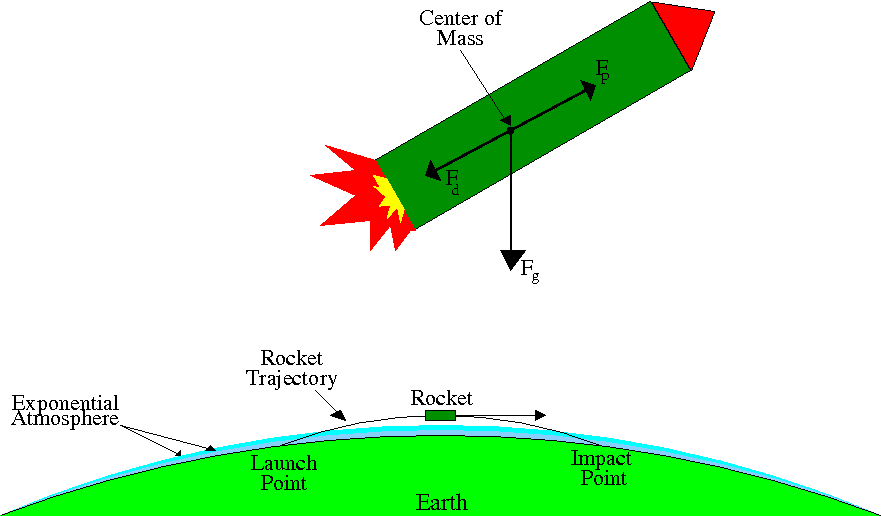
\includegraphics[width=3.25in]{tet.png}}
\caption{\it \small{Force diagram of rocket \label{fig1}}}
  \end{center}
\end{figure}

Figure 1 is a crude depiction of the projectile in this experiment.  From the force diagram above one can see 
the direction of each force vector.  The drag force opposes the motion of the rocket while the force from thrust 
is in the same direction as the rockets motion.  As expected, the force from gravity points towards the center of 
Earth.


\section{Results}

\begin{figure}[H]
 \centerline{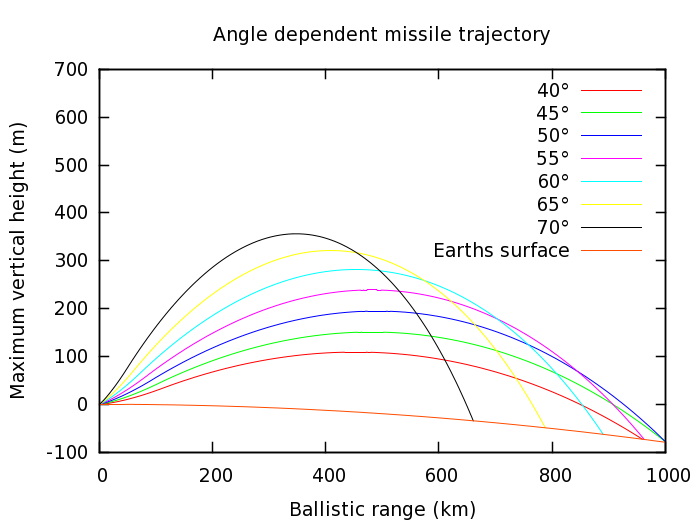
\includegraphics[width=3.0in]{trajectory2.png}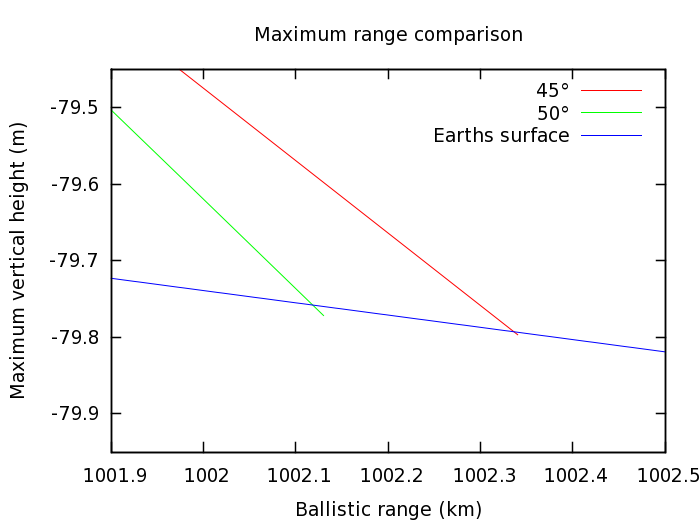
\includegraphics[width=3.0in]{trajectoryzoom3.png}}
\caption{\it \small{Missile trajectory with launch angle dependency \label{fig2}}}
\end{figure}

Depicted, on the left, in figure two are the trajectories of the missile as launched with varying inital angle.  
The inital angle values denoted in the figures key are taken from the horizontal.  The graph on the right is a 
comparison of angles that achieve maximum range.

\begin{figure}[H]
  \begin{center}
\centerline{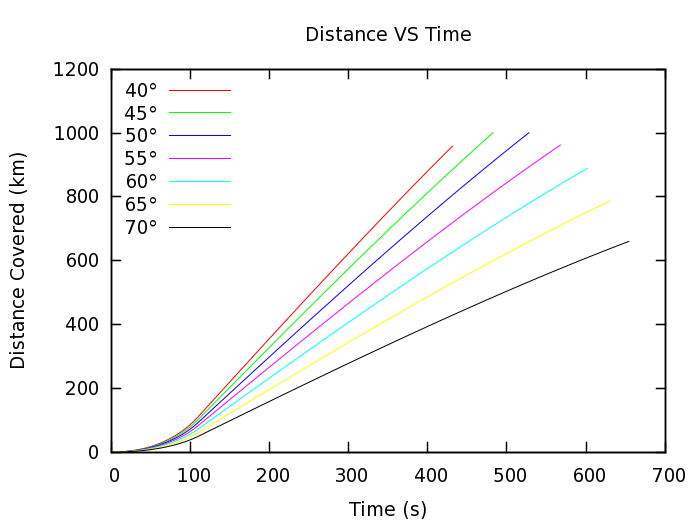
\includegraphics[width=3.5in]{xdistance.png}}
\caption{\it \small{Distance traveled over the ground as a function of time \label{fig3}}}
  \end{center}
\end{figure}

Figure 3 also shows that a missile fired at an angle of 45 degrees will travel~downrange~the~most.

\begin{figure}[H]
  \begin{center}
\centerline{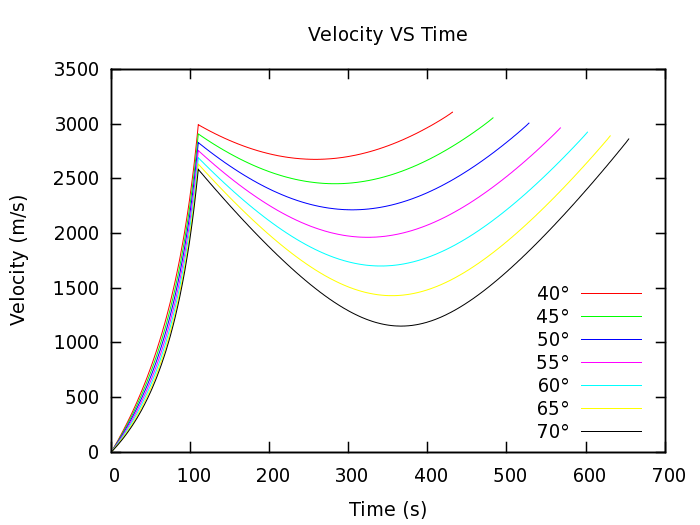
\includegraphics[width=3.75in]{velocity.png}}
\caption{\it \small{Magnitude of the rockets velocity as a function of time \label{fig4}}}
  \end{center}
\end{figure}


\section{Analysis}

In order to achieve a maximum range this projectile must be fired at an angle of 45 degree from the launch surface.  
Figure 3 shows the distance traveled over the ground by the missile, as fired from various angles above the horizontal.  
Outside of the depicted angular range (40-70 degrees) the program breaks down.  Due to gravitational dependencies such a 
simplified program is unable to accurately depict the missile lauched with and inital angle outside of this range.  Using the 
inital launch parameters on the No-Dong missile allowed for the comparison of our results to published data.  The modeled No-Dong 
missile achieved a maximum range of just over 1000 km.  The maximum published range of the No-Dong missile, 700 - 1000 km, agrees 
with our results [3].  The trajectory parameters that give this maximum range are:
\begin{center}
 thrust: p = 26,051 kg
\end{center}

\begin{center}
 launch mass: $m_{0}$ = 16,000 kg
\end{center}

\begin{center}
 initial fuel mass: $m_{fuel}$ = 12,912 kg
\end{center}

\begin{center}
 burn time: $t_{b}$ = 110 s
\end{center}

\begin{center}
 diameter: 1.32 m
\end{center}

\begin{center}
 drag coefficient: $C_{d}$ = 0.25
\end{center}



Figure 4 models the magnitude of the projectile's velocity as a function of time.  At 110 seconds the burn ends, this is 
depicted by the local maximum in figure 4.  From this point on the rocket enters free-fall.  Eventually the acceleration 
due to gravity causes the rocket to change direction and begin its descent.  This transition occurs at the local minimum 
in figure 4.  The overall magnitude of the velocity begins to increase after this point, until the rocket reaches the 
impact point.



\section{Conclusion}
It is evident that a 45 degree angle achieves maximum downrange distance.  Although simplifications were made, the program 
written to model a projectiles behavior do exceedingly well for the necessary range of angles.  You can not ignore the 
effects that occur when the missile passes through the jet stream.  The wind velocity in the jet stream causes a change 
in air density that is taken into account by interpolation atmospheric data.  Any cross wind caused by the jet stream 
alters the path and velocity of the rocket.  If one ignores the curvature of the Earth inaccurate results are achieved.  
Not accounting for the curvature of the Earth alters the landing point of the rocket.  This causes a missile launched at 
a different inital angle to achieve the largest maximum range. 


% the following \setlength is to force the bibliography to have no
% paragraph indentations.Can use vairous units--cm are used here.
\setlength{\parindent}{0cm}

\begin{thebibliography}{99}  % the trailing 99 controls some obscure format--just use

\bibitem{Landau} R. H. Landau and M. J. Paez, "Computational Physics, Problem Solving with Computers," (Wiley: New York) 1997.


\bibitem{Gorham} Gorham, Peter. "Physics 305 Differential Equations." P305lab7. Phys.hawaii.edu, 6 March 2015. Web. 4 Apr. 2015.

\bibitem{nodong} Vick, Charles P. "No-Dong." No-Dong 1 - North Korea. N.p., 17 Feb. 2015. Web. 06 Apr. 2015.

\end{thebibliography}

\section*{Acknowledgements}
All programs developed in modeling the motion of this projectile were written with the aid of Landau [1] and Gorham [2].  
I would like to thank James Ou for his help in reading in the atmospheric data and initalizing it into arrays.



\end{document}

